\documentclass{article}
\usepackage{graphicx}
\usepackage{hyperref}

\title{Homework 1: Game of Life}
\author{Zachary Heras}

\begin{document}
	\maketitle
	
	\section{Problem Statement}
	The goal of this assignment is to develop a sequential program that simulates John Conway's \textit{Game of Life}, which will later be compared to a parallelized version also developed as part of the parallel and concurrent programming course at Rowan University. The program must accept a single input specifying the grid size, \(N\) (where the grid is \(N\) by \(N\)), along with another input for the maximum number of iterations the game is allowed to run. The program's execution time will be evaluated based on a set of test cases provided by the course instructor, Dr. Guo. The program is to be written in C and executed on Rowan University's cluster computer.

	\section{Program Design}
	To begin the program design, a 2D representation of the game board was created using pointers. A pointer to an matrix of integers was used so that the board's size could be dynamically specified during runtime. The internal representation of the game board was \(N+2\) by \(N+2\) to account for the ghost cells needed for boundary wrapping.
	
	Next, functions for handling game board initialization and ghost cell updates were implemented. These functions will not be described in detail, as their implementation is straightforward.
	
	Next, a function to handle game board updates was made. The function loops through each non-ghost cell and checks if the cell should be alive in the next iteration. This is accomplished by counting the number of alive neighbors around each cell, and then going through three if statements to determine the cell's status.
	The first if statement checks if there is exactly three alive neighbors. If this is true, then the cell is alive in the next iteration, regardless of whether it was previously alive or dead. Next, we check if the cell in question is dead. Given the previous statement, if it is dead, then it must be dead in the next iteration. Finally, we check if the cell has exactly two neighbors. If it does, then the cell is alive in the next iteration. Otherwise, the cell is dead in the next iteration. With these three if statements in the aforementioned order, we can correctly assign the cell's alive status. Finally, This function returns true if there was an update anywhere on the game board and false if there was not an update.
	
	From here, the function simply updates the board until the maximum number of iterations is exceeded or until there is no update from one iteration to another.
	
	To compile the program, use the command \texttt{gcc hw1.c -o hw1}, or use the command \texttt{gcc hw1.c -o hw1 -DDEBUG\_PRINT} to print out the game board after each iteration. To run the program, use the command \texttt{./hw1 N I}, where \texttt{N} is the game board side size and \texttt{I} is the number of iterations.

	\section{Test Cases}
	Once the program was made, the next step was to run tests to examine the execution time for each predetermined test. The tests that will be run are shown in Table \ref{table1} below. Each test will be run 3 times and the average execution time will be reported.

	\begin{table}[ht]
		\centering
		\begin{tabular}{|c|c|}
			\hline
			\textbf{Board Size (N x N)} & \textbf{Max Iterations} \\
			\hline
			1000 x 1000 & 1000 \\
			5000 x 5000 & 1000 \\
			5000 x 5000 & 5000 \\
			10000 x 10000 & 1000 \\
			10000 x 10000 & 10000 \\
			\hline
		\end{tabular}
		\caption{Tests with board size and max iterations.}
		\label{table1}
	\end{table}

	\section{Test System Configuration}
	Each test was executed on the Rowan cluster computer, utilizing one of the \texttt{csm-com-[001-012]} nodes. A Slurm script was written for each test to preserve the test setup information. The scripts were stored in \texttt{.sh} files, following the naming pattern \texttt{run\_hw1\_x\_y.sh}, where \texttt{x} represents the test case and \texttt{y} represents the test number.

	
	\section{Analysis and Conclusions}
	Below, figure \ref{figure1} and table \ref{table2} describing the resulting execution times. The figure displays the \(\log_{10}\) of the execution times for each test case 1-5. From both the table and the figure, we see an exponential growth in execution time as the size of the game board increases. In the case where the maximum number of iterations was capped at 1000 for the \(1000\) by \(1000\) board, the experiment seems to have been terminated due to reaching the iteration limit, as its execution time was lower than that of the \(5000\) by \(5000\) board, which had a larger iteration limit.
	
\begin{figure}[t]
    \centering
    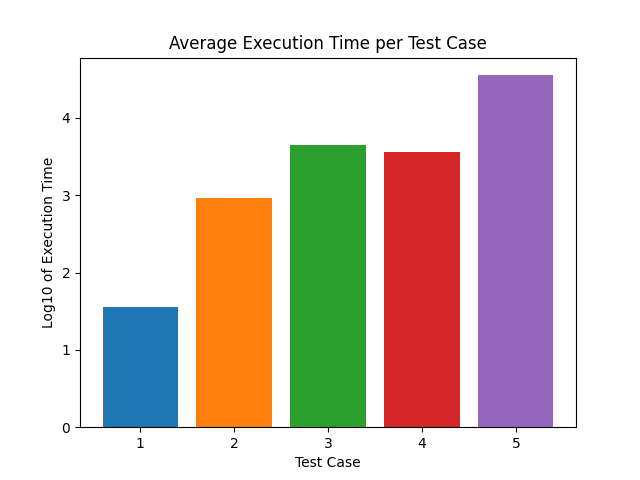
\includegraphics[width=0.8\textwidth]{average_execution_time_per_test_case}
    \caption{Average Execution Time per Test Case.}
    \label{figure1}
\end{figure}

	
	\begin{table}[t]
		\centering
		\begin{tabular}{|c|c|c|}
			\hline
			\textbf{Board Size (N x N)} & \textbf{Max Iterations} & \textbf{Average Execution Time (s)} \\
			\hline
			1000 x 1000 & 1000 & 36 \\
			5000 x 5000 & 1000 & 913 \\
			5000 x 5000 & 5000 & 4450 \\
			10000 x 10000 & 1000 & 3663 \\
			10000 x 10000 & 10000 & 35571 \\
			\hline
		\end{tabular}
		\caption{Tests with board size and max iterations.}
		\label{table2}
	\end{table}
	
	\section{References}
	\begin{itemize}
		\item https://www.w3schools.com/c/
	\end{itemize}
	
\end{document}